\documentclass[10pt,letterpaper]{article}
\usepackage[top=0.85in,left=2.75in,footskip=0.75in]{geometry}

% Use adjustwidth environment to exceed column width (see example table in text)
\usepackage{changepage}

% Use Unicode characters when possible
\usepackage[utf8]{inputenc}

% textcomp package and marvosym package for additional characters
\usepackage{textcomp,marvosym}

% fixltx2e package for \textsubscript
\usepackage{fixltx2e}

% amsmath and amssymb packages, useful for mathematical formulas and symbols
\usepackage{amsmath,amssymb}

% cite package, to clean up citations in the main text. Do not remove.
\usepackage{cite}

% Use nameref to cite supporting information files (see Supporting Information section for more info)
\usepackage{nameref,hyperref}

% line numbers
\usepackage[right]{lineno}

% ligatures disabled
\usepackage{microtype}
\DisableLigatures[f]{encoding = *, family = * }

% rotating package for sideways tables
\usepackage{rotating}

% Remove comment for double spacing
%\usepackage{setspace} 
%\doublespacing

% Text layout
\raggedright
\setlength{\parindent}{0.5cm}
\textwidth 5.25in 
\textheight 8.75in

% Bold the 'Figure #' in the caption and separate it from the title/caption with a period
% Captions will be left justified
\usepackage[aboveskip=1pt,labelfont=bf,labelsep=period,justification=raggedright,singlelinecheck=off]{caption}

% Use the PLoS provided BiBTeX style
\bibliographystyle{plos2015}

% Remove brackets from numbering in List of References
\makeatletter
\renewcommand{\@biblabel}[1]{\quad#1.}
\makeatother

% Leave date blank
\date{}

% Header and Footer with logo
\usepackage{lastpage,fancyhdr,graphicx}
\graphicspath{ {/figures/} }
\usepackage{epstopdf}
\pagestyle{myheadings}
\pagestyle{fancy}
\fancyhf{}
\lhead{
\includegraphics[width=2.0in]{PLOS-submission.eps}}
\rfoot{\thepage/\pageref{LastPage}}
\renewcommand{\footrule}{\hrule height 2pt \vspace{2mm}}
\fancyheadoffset[L]{2.25in}
\fancyfootoffset[L]{2.25in}
\lfoot{\sf PLOS}

\usepackage[section]{placeins}

%% Include all macros below

\newcommand{\lorem}{{\bf LOREM}}
\newcommand{\ipsum}{{\bf IPSUM}}

%% END MACROS SECTION


\begin{document}
\vspace*{0.35in}

% Title must be 250 characters or less.
% Please capitalize all terms in the title except conjunctions, prepositions, and articles.
\begin{flushleft}
{\Large
\textbf\newline{Delineate urban boundaries in Great Britain from the network of Twitter user spatial interactions}
}
\newline
% Insert author names, affiliations and corresponding author email (do not include titles, positions, or degrees).
\\
Junjun Yin\textsuperscript{1, 2, 3},
Aiman Soliman\textsuperscript{1, 2, 4},
Dandong Yin\textsuperscript{1, 2, 3},
Shaowen Wang\textsuperscript{1, 2, 3, 4, $\ast$}
\\
\bigskip
\bf{1} CyberGIS Center for Advanced Digital and Spatial Studies
\\
\bf{2} CyberInfrastructure and Geospatial Information Laboratory (CIGI)
\\
\bf{3} Department of Geography and Geographic Information Science
\\
\bf{4} National Center for Supercomputing Applications
\\
\bf{} University of Illinois at Urbana-Champaign, 61801, IL, USA
\\
\bigskip

% Insert additional author notes using the symbols described below. Insert symbol callouts after author names as necessary.
% 
% Remove or comment out the author notes below if they aren't used.
%
% Primary Equal Contribution Note

% Current address notes
%\textcurrency a Insert current address of first author with an address update
% \textcurrency b Insert current address of second author with an address update
% \textcurrency c Insert current address of third author with an address update

% Deceased author note
%\dag Deceased

% Group/Consortium Author Note
%\textpilcrow Membership list can be found in the Acknowledgments section.

% Use the asterisk to denote corresponding authorship and provide email address in note below.
* shaowen@illinois.edu

\end{flushleft}
% Please keep the abstract below 300 words
\section*{Abstract}
Urban regions are discrete urban areas with various social-economic relations and commute patterns of citizens.
Defining boundaries of the urban regions are of great importance for city planning, traffic management and resource allocation.
As existing urban boundaries are usually defined by government political and administrative purposes, it is not clear whether they truly reflect people daily interactions with the urban spaces, such as intra- and inter regional activities?
In this study, we presented a natural way for redrawing the urban boundaries based on human interactions with the physical spaces.
To be specific, we delineated the urban boundaries in Great Britain from a network of large-scale Twitter user spatial interactions, which were inferred from more than 69 million Twitter messages.
Our study provides a first step in connecting human mobility research with defining natural urban boundaries based on Twitter user spatial interactions, which provides a new perspective for understanding the interactions between urban structures with human activities. 
We redrew the natural boundary in a hierarchical fashion based on different range of user physical movements as it was inferred from the collective mobility patterns of the captured Twitter users in Great Britain.
The results of strongly connected urban regions in the form of communities in the network space yielded geographically cohesive, non-overlapping urban areas, which provides a clear delineation of the urban boundaries in Great Britain.
The technique was applied to both national level (Great Britain) and city level (greater London region), while the results corresponded well to the administrative boundaries, some of the unexpected and interesting boundaries were identified.

\linenumbers
\section*{Introduction}
Today’s urban boundaries (i.e. edges and districts) are usually defined by government agencies for political and administrative purposes.
While urban environments are conceptualized as spaces that are recreated and formed by human activities~\cite{schliephake}, a fundamental question for this “top-down” based approach to defining urban boundaries is whether it reflects the empirical humans interactions across space, such as commuting or trading activities between the borders.
Further, urban boundaries that respect how people naturally interact with the space can be of great importance for city planning, traffic management and resource allocation~\cite{lynch1960,jiang2015,liu2015,long2015}.
Many studies have adopted a ``bottom-up” approach for delineating urban boundaries, where the geographic space is partitioned into small units and each unit is modeled as a node in a network.
Then a suitable community detection algorithm is applied to partition the network and associated geographic space based on the strength of human interactions among them~\cite{lancichinetti2009}.
Different social and physical human interaction were considered to establish the edges of the network between nodes.
For example, a large set of telephone call records were used to represent the network of human interaction across space and delineated urban boundaries in Great Britain~\cite{ratti2010}.
Extended the previous method to different countries~\cite{sobolevsky2013}, the authors argue that this method yields cohesive geographic divisions that follow the socio-economic boundaries. 
While~\cite{kallus2015} have used social ties of Twitter users to identify cohesive regions for different countries across the world, where the authors found evidence for dividing due to local conflicts and cross-countries uniting trends to further support the ``bottom-up" approach to mapping natural boundaries.

In this study, we describe a novel approach to delineate urban boundaries based on the Twitter user movements extracted from massive Twitter dataset, with more than 69 million Twitter messages from $1^{st}$ June to $31^{st}$ December, 2014.
Geo-located Twitter data is proven to be a useful source for studying human mobility patterns at a large spatial scale, for example, country level~\cite{hawelka,jurdak2015}.
We argue here that Twitter user mobility patterns provide a different view of natural units based on physical commuting rather than social ties or phone call initiation. 
A unique advantage is to delineate natural urban boundaries in a hierarchical fashion based on different range of user physical movements, which are inferred from the collective mobility patterns of the captured Twitter users in Great Britain. 
In addition, Twitter data are not sensitive to user privacy issues nor have a spatial granularity that is limited to zip code level~\cite{thiemann}, which can only produce sparse delineation.

We delineated the geography of urban boundaries in Great Britain by imposing a virtual fishnet over the islands of Great Britain. 
Twitter user movements were used to establish the connections between the virtual fishnet cells and form the connectivity network, where each cell acts as a node in a network.
We applied the map equation algorithm~\cite{domenico2015} to partition the network,  and associated geographic regions.
The map equation algorithm was selected to avoid the inherent resolution problem~\cite{fortunato2007} of the common modularity maximization method~\cite{newman2006}. 
We found that the collective mobility patterns of Twitter users in Great Britain are divided into several distance ranges starting from short intra-city to inter-city movements with clear distinction points. 
Identifying the connected regions at each of these distance ranges yielded a hierarchical boundaries of  the urban space in Great Britain.
Our study provides a first step in connecting human mobility research with defining natural urban boundaries based on Twitter user spatial interactions. It provides a new perspective for understanding the interactions between human activities with urban structures. 

\section*{Materials and Methods}
\subsection*{Overview}
Our motivation of this study is to utilize large-scale Twitter user spatial interactions, which are inferred from the collective mobility patterns of Twitter users, to delineate urban boundaries in Great Britain.
In particular, a Twitter user's movement refers to the individual's relocation or displacement~\cite{gonzalez2008} in the geographic space.
It is not equivalent to a ``trip" took by an individual, for instance, even the time interval between two recorded locations is one month, it still counts as a displacement.
To identify the clusters of urban regional connectedness via large-scale Twitter user movements, we first imposed a virtual fishnet over the islands of Great Britain, where Twitter user movements were used to establish the connections between the virtual fishnet cells and form the connectivity network with each cell acts as a node in a network. 
Finally, by detecting strongly connected clusters in the network space with community detection methods~\cite{coscia2011}, the urban boundaries of these clusters were revealed back in the geographic space. 
An overview of the approach is illustrated in Fig.~\ref{S1_Fig} and the details are presented in the following sections. 

\begin{figure}[ht]
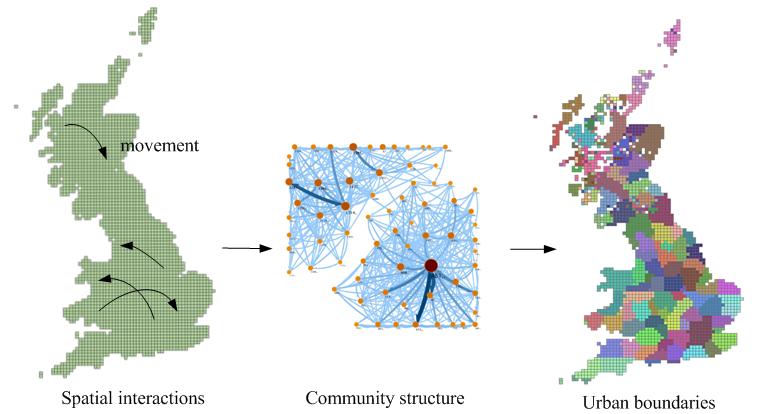
\includegraphics[width=1\linewidth]{./figure/PNG/S1_overview_Fig_2}
\caption{{\bf An overview for delineating urban boundaries from Twitter user movements}}
\label{S1_Fig}
\end{figure}

\subsection*{Geo-located Twitter Data}
A geo-located tweet is a Twitter message appended with an additional geo-tag expressed as a pair of geographical coordinates that represents the location from which the tweet was sent.
In this study, the geo-located tweets were collected using the Twitter Streaming API (\url{https://dev.twitter.com/streaming/overview}) by supplying a geographical bounding box as an area-of-interest to retrieve all the contained geo-located tweets.
To ensure complete coverage of Great Britain, we set the bounding box to British Isles using the lower left and upper right coordinates (49.497, -14.854), (61.186, 2.637). This does include the whole of Ireland and part of France.
We have implemented a data crawler and continuously collected 7-months of data ($1^{st}$ June – $31^{st}$ December, 2014) resulting in over 101.8 million tweets at 60 GB in size. 
To showcase the overall spatial coverage of the collected geo-located tweets, a density map of the Twitter user locations in British Isle for July 2014 is shown in Fig.~\ref{S2_Fig}, where the collected points visualization reveals the geography of cities. Notice the clusters with higher densities of tweets (in color red) correspond to the locations of major cities.

\begin{figure}[ht]
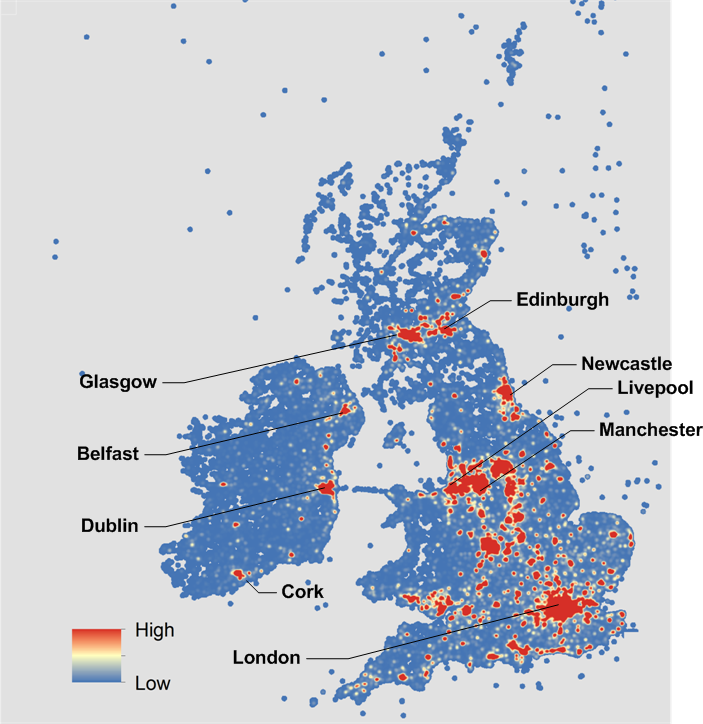
\includegraphics[width=0.7\linewidth]{./figure/PNG/S2_twitter_density_Fig_1}
\caption{{\bf The density map of the Twitter user locations for July 2014}}
\label{S2_Fig}
\end{figure}

To verify the collected tweets are from human users, the raw tweets were further filtered by the following steps. 
First we removed the duplicated messages in the dataset.
Next, we removed non-human users based on unusual relocation speed \cite{hawelka,jurdak2015}. 
We adopted a relocation speed threshold of 240 m/s as used in \cite{jurdak2015}. 
We examined all the consecutive locations of each user and excluded those with relocating speed above the threshold.
Because the original location information embedded in the geo-tag is given in units of latitude and longitude, we projected the points into British National Grid (EPSG: 27700) coordinate system for the ease of distance calculations. 
Finally, we used the geographical boundary of Great Britain, which is derived from Office for National Statistics (ONS) of UK (\url{http://www.ons.gov.uk/ons}), to further restrict the remaining tweets to be ``domestic".
Based on these reinforcements, the filtered dataset for the following study contains 69,847,497 tweets from 1,153,891 users.

At this stage, each geo-located tweet is represented as a tuple $\langle user\_id, loc, t, m \rangle$, where $user\_id$ is an anonymous Twitter user’s id; $loc$ is the recorded location of the tweet as a pair of coordinates; $t$ is the timestamp of when the tweet was posted; and $m$ is the actual content of the tweet. 
To protect Twitter users’ privacy, the id field was replaced with a randomly generated unique number. 
Because we are interested in the collective Twitter user movements instead of individual user trajectories, the content of the message was removed. 
This simplifies the geo-located tweets and can be shared with other researchers upon request.

\subsection*{A network of large-scale Twitter user spatial interactions}
Urban regions are discrete urban areas, with various social-economic relations and commute patterns of citizens. 
In this connection, certain urban regions are more strongly connected to other urban regions than others.
Therefore, in this study, a connection is built between two urban regions when one of them is the origin of a Twitter user’s movement and the other is the destination. 
Such connections can be represented by an origin-destination (OD) matrix based on the collective Twitter user movement flux within the time span (i.e., $1^{st}$ June – $31^{st}$ December, 2014). 
This OD matrix is essentially a mathematical representation of a weighted directed graph $G\equiv\langle V, E_{w}\rangle$ where $V$ is a set of spatial nodes corresponding to the underlying urban regions; and $E_{w}$ is a set of edges representing the connections between a pair of nodes and the corresponding weights are assigned as the accumulated volume of Twitter user movement between the two urban regions.

To build such a spatial network at a national level, one must determine the basic units as the spatial nodes for mapping and aggregating the movement flows. 
Previous studies have suggested spatial tessellation as mapping units, which uses voronoi polygons to partition the space based on the collected points~\cite{rinzivillo2012,zhong2014}. 
This approach demonstrates improvements for estimating the locations of mobile phone records based on the cell tower triangulation~\cite{gonzalez2008,qian2013}.
However, it actually decreases the spatial resolution for geo-located tweets, as the location information is usually derived from the embedded GPS in the mobile devices and tends to provide better accuracy~\cite{sakaki2010,zandbergen2009}.
Another popular approach is to partition the space into a grid of spatial pixels~\cite{liuPopMobility,ratti2010}.
However, deciding the size of the cell can potentially encounter the Modifiable Areal Unit Problem (MAUP)~\cite{openshaw1984,wong2009}, where different choices of unit size can lead to significant variant findings.
To compare our investigation with the findings in similar studies but avoiding subjectively deciding the cell size, we performed statistical analysis of Twitter user mobility patterns in Great Britain measured by the distribution of collective Twitter user displacements and radius of gyrations of individuals \cite{gonzalez2008,jurdak2015}.

In particular, as radius of gyration is a metric to distinguish mobility patterns of individuals~\cite{gonzalez2008}, which is defined as Eq. \eqref{eq:2}:
\begin{equation} \label{eq:2}
r_{g} = \sqrt{\frac{1}{n}\sum_{i=1}^{n}(p_{i} -  p_{centroid})^{2}}, \textrm{where}\hspace{1ex} p_{centroid} = \frac{1}{n}\sum_{i=1}^{n}p_{i}
\end{equation}

\noindent It measures the accumulated distances of deviation from the center of mass of an individual user's trajectory, where $p_{i}$ is one of the user's locations and $p_{centroid}$ is the center of mass of the user's trajectory.
By examining the probability distributions of radius of gyrations, also known as the spatial dispersal kernel $P(r_g)$~\cite{brockmann2006}, we chose 10 km as the cell size, which is the value for quantifying the spatial coverage from majority of Twitter users in Great Britain (Fig.~\ref{S4_Fig} - c, with details shown in the next section). 
In this case, we have created a fishnet with 2784 10-km size cells.
The cells within the fishnet act as proxies for representing individuals' spatial coverage areas, which focus more on the inter-connections among cells to identify the strongly connected clusters. 

\subsection*{Community structure of the spatial networks}
Based on the derived spatial network, which is a directed weighted graph, we further determined the clusters of strongly connected spatial nodes, also known as communities in the graph space~\cite{coscia2011}. 
There are a variety of community detection algorithms, which can produce different results depending their definition of community in the network~\cite{coscia2011}.
A common usage of community detection is based on modularity maximization~\cite{newman2006}, such as the previous studies in~\cite{hawelka,ratti2010,song2012}.
However, such an approach is often problematic: it is found to have an inherent resolution problem, where small communities are either ignored~\cite{fortunato2007} or assigned with high modularity scores \cite{guimera2004}; it is also found to produce less informative partitions in many empirical networks~\cite{good2010}.
Since our graph is a directed weighted graph, the alternative community detection library found from the literature is Infomap~\cite{domenico2015,rosvall2008}, which was considered to produce better community detections~\cite{lancichinetti2009}.

The Infomap uses the map equation~\cite{rosvall2010} for representing the probability of flow of random walks in information systems.
It finds communities by minimizing the expected description length of the trajectory of a random walker, which is shown below:
\begin{equation} \label{eq:1}
L(M)=qH(Q) + \sum_{i=1}^{m} p_{i}H(p_{i})
\end{equation}

In Eq. \eqref{eq:1} , $L(M)$ consists of two terms: qH(Q) is the entropy of the movements among clusters and $ \sum_{i=1}^{m} p_{i}H(p_{i})$ is the entropy of movements within clusters. 
To be more specific, q is the probability of a random walker jumps from one cluster to another, while $p_i$ is the probability of in-cluster movements in cluster i.
In this regard, this algorithm can be intuitively tailored to describe the context of finding strongly connected clusters of urban regions (i.e., spatial nodes) based on  Twitter user movements.
The detailed literatures and implementations of Infomap can be found from this website (\url{http://mapequation.org}).
Note that Infomap is capable of performing multi-level community detections~\cite{domenico2015}, but we only use the algorithm to produce most detailed community structures
to examine groups of strongly connected urban regions.

\section*{Results and Discussion}
\subsection*{Collective Mobility Patterns of Twitter Users in Great Britain}
We first modeled different aspects of the collective mobility patterns of Twitter user (i.e., number of visited locations per user,  collective user displacements and radius of gyration of individuals) in order to identify natural breaks in the user travel patterns.
Furthermore, we used these natural breaks of mobility patterns to partition the geographic space of Great Britain into a fine-grained cells and establish the connectivity among these cells to redraw natural urban boundaries. 

We found that the cumulative distribution function~\cite{clauset2009} of the number of locations visited by each Twitter user during the timespan (1$^{st}$ June – 31$^{st}$ Dec, 2014) follows a two-tier power law distributions (shown in Fig.~\ref{S3_Fig}). 
The majority (the front part) of the distribution follows a truncated power-law distribution $P(X\geq x)\sim x^{-\alpha}e^{-\lambda x}$, where $\alpha = 1.24, \lambda =0.00132$; and the tail part (less than 2$\%$ of the whole population) follows a power-law distribution  $P(X \geq x)\sim x^{-\alpha}$ with $\alpha$ value is 3.2.
The distribution was found to be consistent over all individual months (June to December, 2014), which has a slight offset in the truncated power-law distribution with the mean $\alpha$ value as 1.26 $ \pm$  0.05 (standard deviation) and the mean $\lambda$ value as 0.00134 $ \pm$  0.0002 (standard deviation). 

The two-tier power law distribution indicates that the collective behaviors of Twitter user visiting different locations can be well approximated with a (truncated) L\'{e}vy Walk (a random walk) model~\cite{rhee2011,reynolds2012}, which has also been identified in many human mobility studies using different mobility data~\cite{zhao2015}.
The similarities among the distributions suggest that the mobility data collected from geo-located tweets are temporally stable, at least at the monthly interval, which indicates our approach of using Twitter user mobility to delineating urban boundaries is not a snapshot of the whole process.  
In addition, the L\'{e}vy Walk model reveals the diversity regarding the number of visited locations per user, which indicates a level of ``randomness'' in Twitter user movements across space. 
It in turn justifies our choice of using the map equation community detection algorithm~\cite{rosvall2008} to identify the clusters of urban regional connectedness via large-scale Twitter user movements.

\begin{figure}[ht]
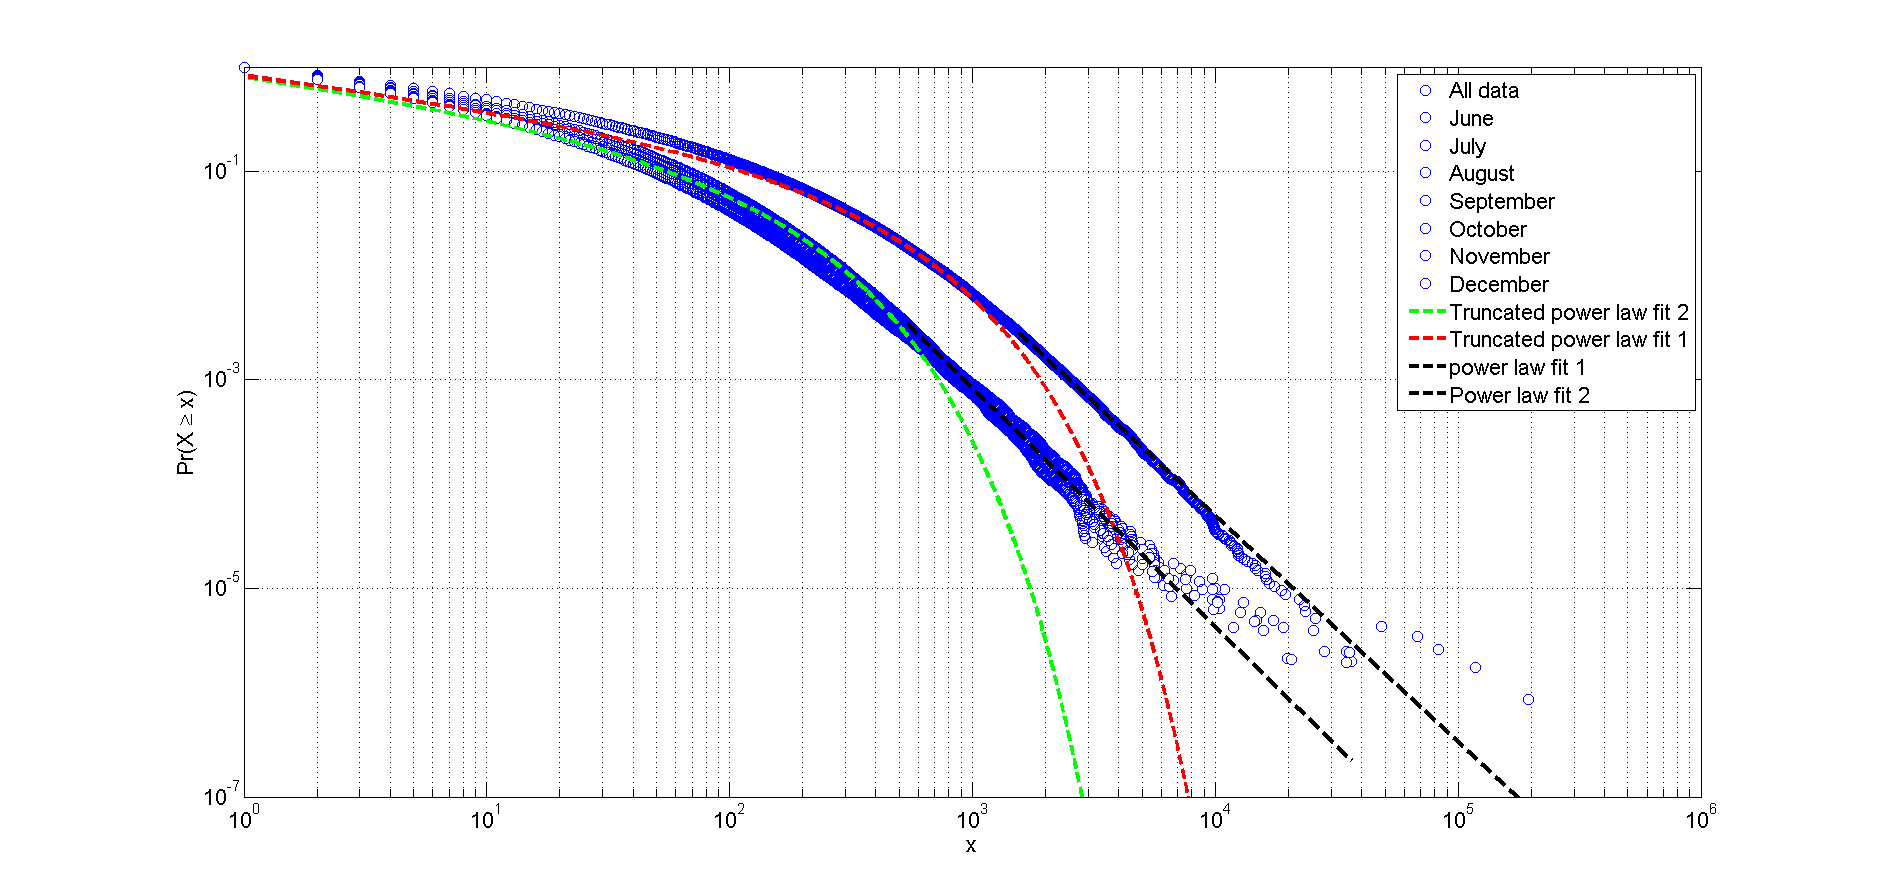
\includegraphics[width=1.0\linewidth]{./figure/PNG/S3_visitation}
\caption{{\bf Cumulative distribution of the number of locations visited by each Twitter user during different timespan}}
\label{S3_Fig}
\end{figure}

We further studied two aspects of Twitter user mobility pattern: the distribution of Twitter user displacements and radius of gyration. 
Twitter user displacement refers to the distance between each two consecutive locations in a user’s trajectory using a “crow's fly distance” (i.e., the direct distance); and the radius of gyration describes the deviation of distance from the center of mass in a user’s trajectory.
The probability distributions of the collective user displacements $P(d)$ and radius of gyration $P(r_g)$ are presented in Fig.~\ref{S4_Fig}, where the fitting method for identifying different distance ranges is derived from~\cite{jurdak2015}.
The probability distribution of the collective displacements can be approximated by $P(d) \sim \lambda_{1} e^{-\lambda_{1}(d - d_{min})}, d_{min}=10m$ from [10m, 70m] (accounting for 3 $\%$ of the population),  $ P(d) \sim \beta\lambda_{1}d^{\beta-1}e^{-\lambda^{1}(d^\beta-d_{min}^\beta)}, d_{min} = 100m$ from [70m, 70km] (93 $\%$ of the population), and $P(d) \sim {d}^{-\alpha}$ [$>$ 70km] (4 $\%$ of the population). 
In particular, the displacement distance between 70m and 100km can be further approximately by two power law distributions with a cutting point at 4km (55$\%$ distances are less than 4km and 40$\%$ distances between 4km and 100km), which indicates the urban movements captured by the geo-located Twitter data reveals two different modes, such as inter- or intra-city movements. 
In summary, these fitting functions suggest the existence of multi-scale or multi-modal urban movements captured from Twitter users in Great Britain, which means the geographically cohesive, non-overlapping urban areas (identified in the next section) are not just a result of short distance movements but naturally emerged from the collective Twitter user mobility pattern.
Note that similar multiphase pattern was observed of Twitter user displacement in Australian but with slightly different distance ranges\cite{jurdak2015}.

Further, we analyzed the distribution of radius of gyration to understand the movement from point of view of individual Twitter users rather than separated displacements.
The distribution of radius of gyration can be approximated by a combination of three functions: $P(r_{g}) \sim \lambda_{2} e^{-\lambda_{2}(r_{g} - {r_{g}}_{min})}, {r_{g}}_{min}=10m$ from [10 m, 30m], $P(r_{g}) \sim \lambda_{2} e^{-\lambda_{2}(r_{g} - {r_{g}}_{min})}$ from [50m, 10km], and $P(r_{g}) \sim {r_{g}}^{-\alpha}$ [10km, 100km], where these three functions account for 92$\%$ of all the users.
This suggests that there are mainly three types of users, where some Twitter users (1) tend to stay at one location or at nearby locations when they tweet, some users (2) tend to move in intra-city scale when they tweet and some users’ (3) movements tend to have a large spatial coverage. 
In particular, (1) and (2) account for approximately 53$\%$ of all users.  
The radius of gyration between 30m and 100km can be further approximately by two power law distributions with a cutting point at 2.5km (35 $\%$ users with radius of gyration less than 2.5km and 57$\%$ users with radius of gyration between 3km and 100km), which suggest two main types of spatial coverage of Twitter user movements in Great Britain. 
Note that the accuracy of these values for defining the distance bound depends on the accuracy of the location information of each geo-located tweet. 
These findings are consistent with the findings in research on human mobilities where the radius of gyration of human movements is bounded to different distance ranges~\cite{brockmann2006,gonzalez2008}.
The distance-decay effects found in both user displacements and radius of gyration show evidences of spatial proximity in Twitter user movements. 
It explains the communities of urban regions in a graph space are geographically close and yet still be able to be separated from other groups, which essentially result in the delineating urban boundaries based on Twitter user spatial interactions.

\begin{figure}[ht]
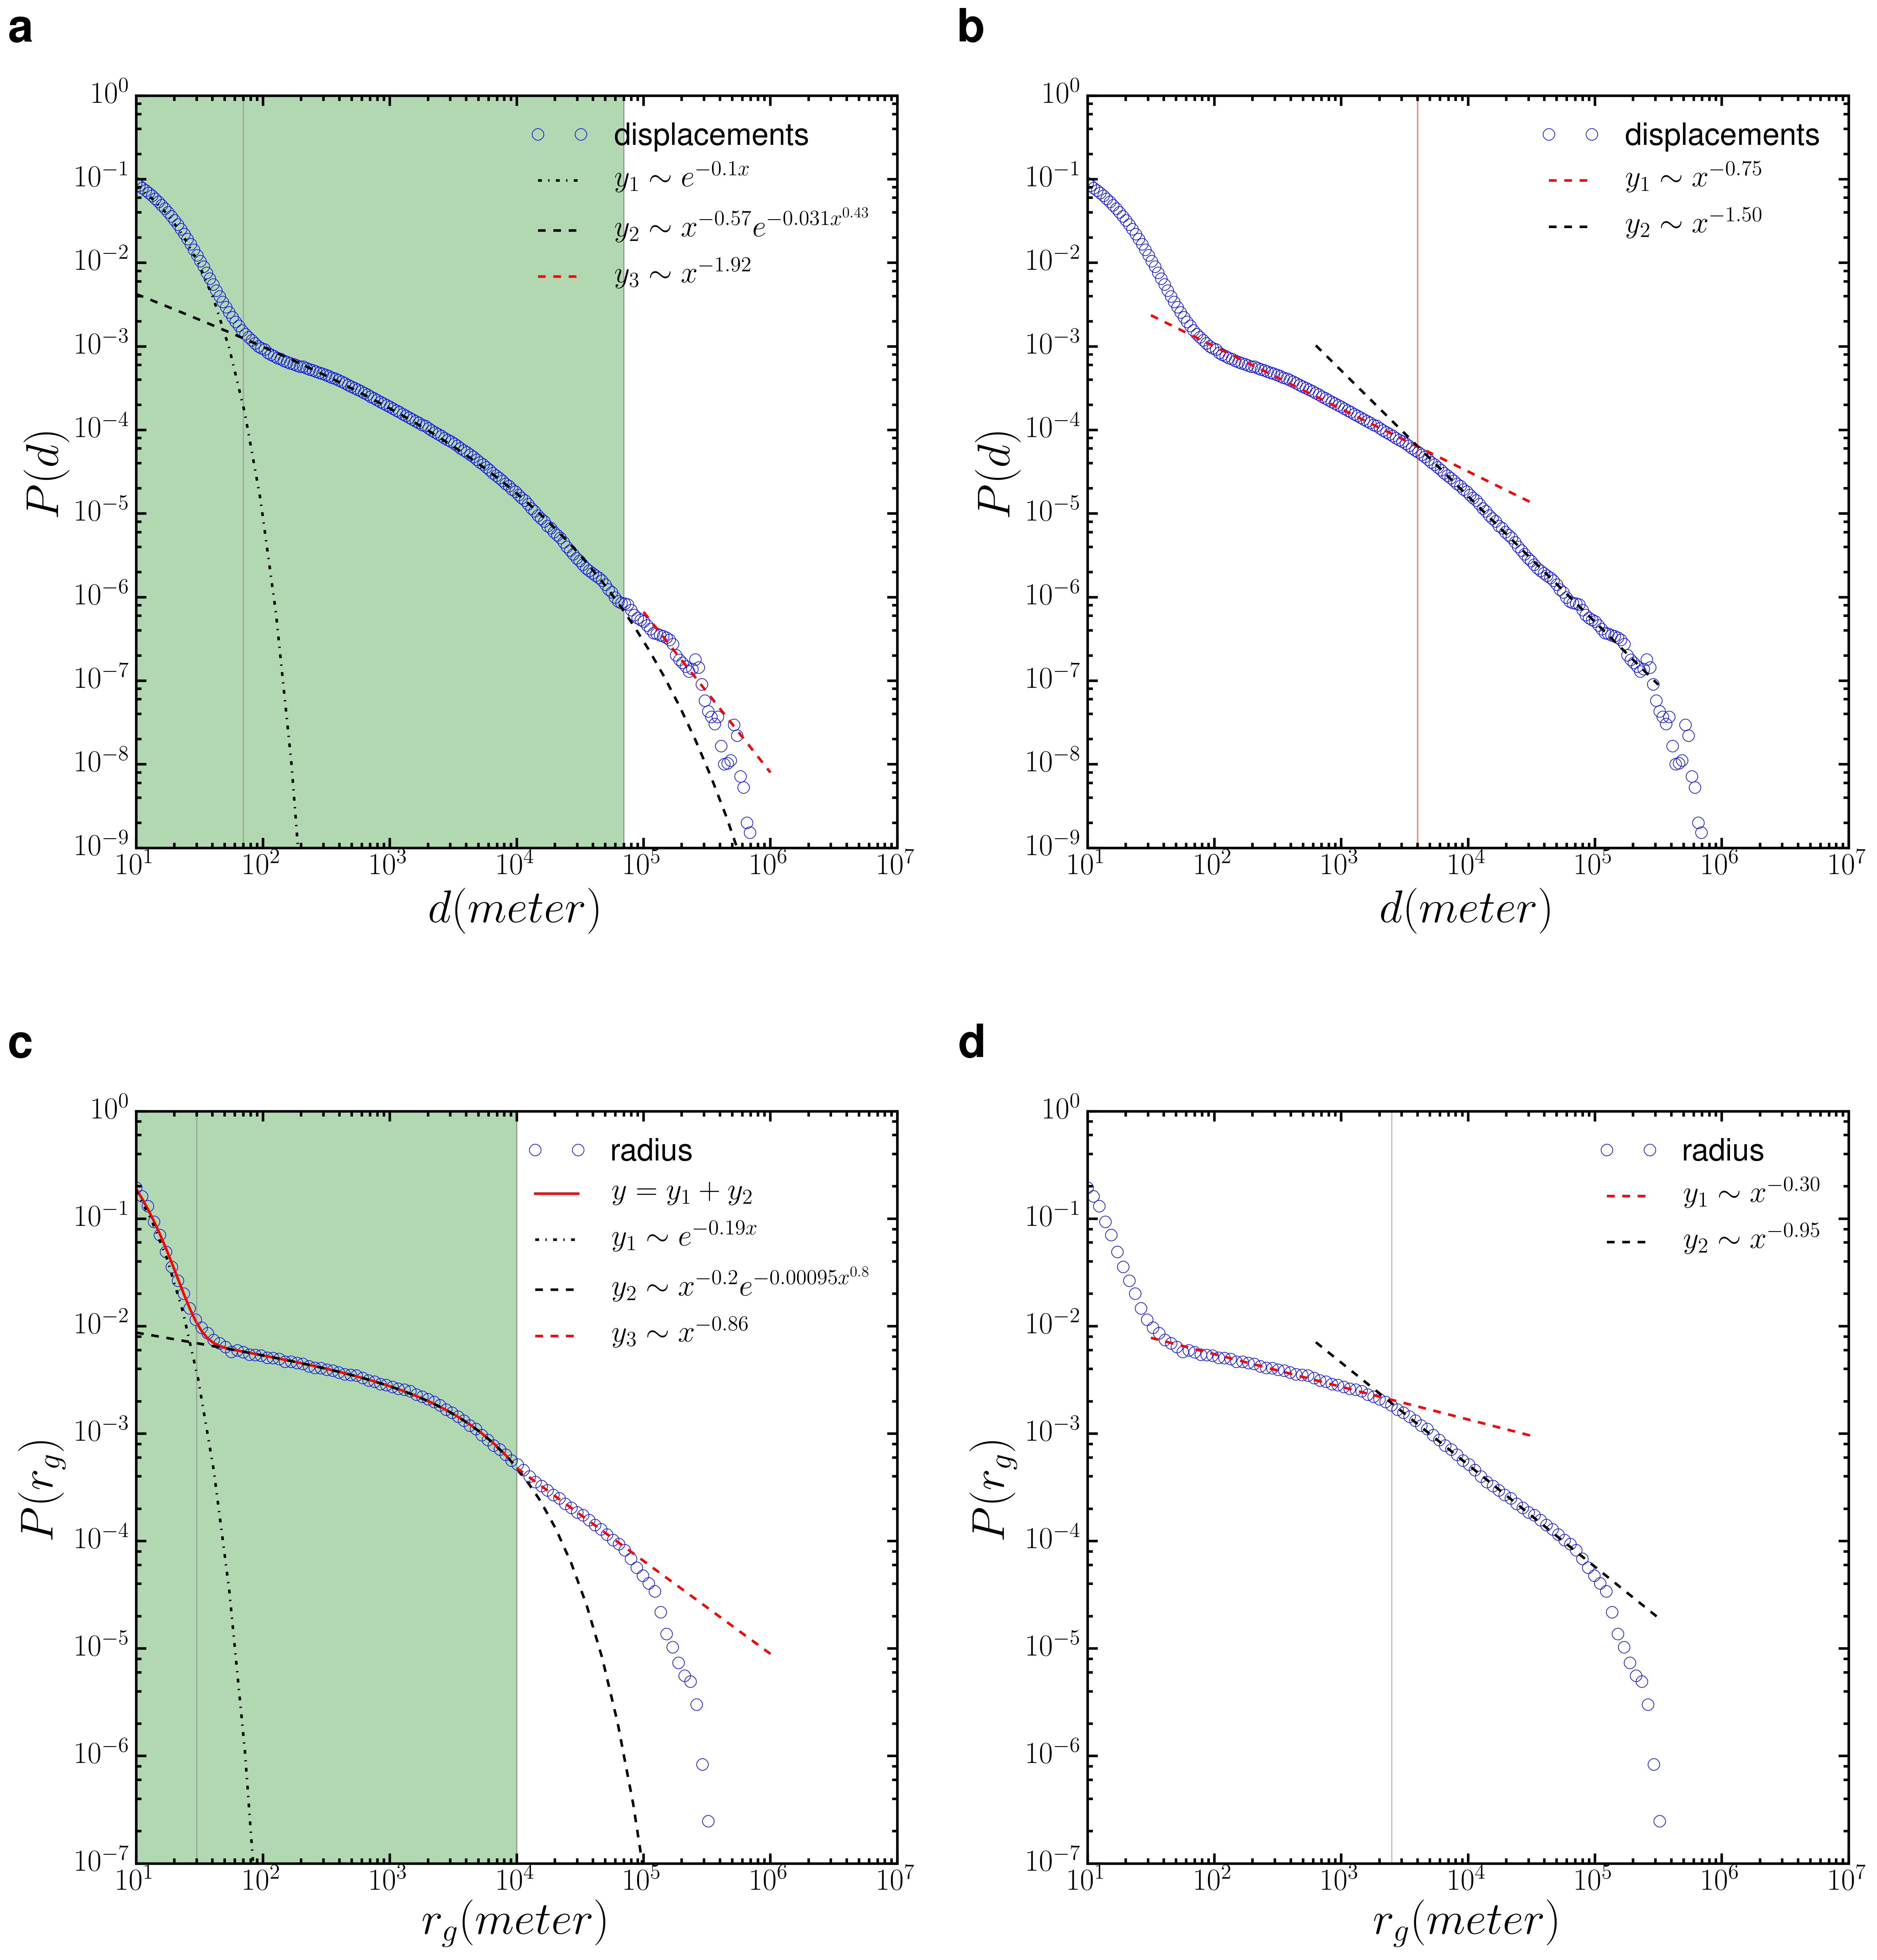
\includegraphics[width=1.0\linewidth]{./figure/PNG/S4_radius_displacement}
\caption{{\bf The probability distribution of Twitter user displacements and radius of gyration:} (a) The displacement distribution $P(d)$ is approximated by an exponential, a stretched-exponential and a power-law function (b) the distance between [70m, 70km] is approximated by a double power-law functions (c) The distribution of radius of gyration $P(r_g)$ is approximated by the combination of an exponential, a stretched-exponential and a power-law function (d) the distance between [30m, 100 km] is approximated by a double power-law functions}
\label{S4_Fig}
\end{figure}

\subsection*{Redefining Great Britain’s Administrative Boundaries}
The network of Twitter user spatial interaction in this study was constructed by nodes represented by 10 km by 10 km fishnet cells, which provides an adequate resolution for country wide investigation~\cite{ratti2010}.
The edges of this network were derived from the number of directed Twitter user movements/displacements between each pair of cells.
We used the connectivity network as a proxy to partition the space associated with its nodes.
Coherent geographic regions were identified as individual fishnet cells showing more inner transportation compared to transportation with the outside cells.
Fig.~\ref{S5_Fig}  presents the delineated urban boundaries based on Twitter user displacement distance less than 4 km, greater than 4km, greater than 10 km and using all available displacements together compared to the administrative boundaries of Great Britain counties.
One clear observation across the coarse and fine delineations is that most of the geographic divisions are centered around big urban cores with relatively high population.
This results is expected given that most of the tweets originates in urban centers.
However, what is remarkable is the performance of this approach in dividing the remaining space between cities.
We found that restricting the trip distance resulted in different delineations of the travelers catchment area around these centers.
For example, one could explain these effects as a manifestation of the underlying gravity law~\cite{simini2012} and the distance decay effect on attracting travelers~\cite{gonzalez2008}.
Remarkably, our approach performed well in terms of dividing the entire space with minimum gaps.
Empty cells were found in regions with no, or few Twitter users had visited (e.g., forests, agriculture) especially in the case of restricting the analysis to short distance Twitter user displacements.

\begin{figure}[ht]
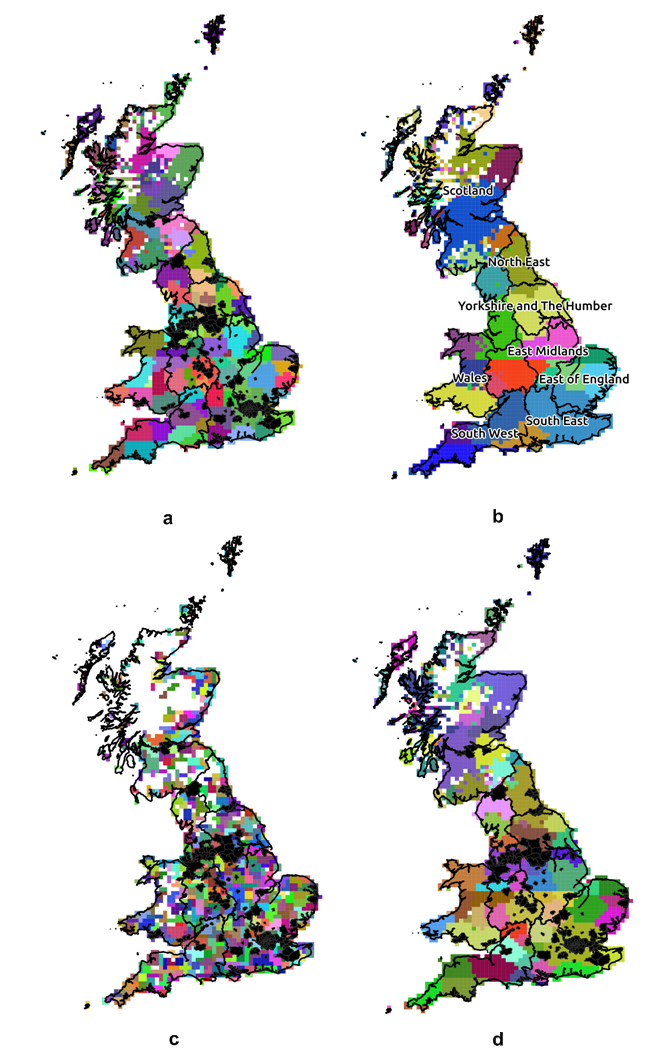
\includegraphics[width=0.9\linewidth]{./figure/PNG/S5_community}
\caption{{\bf The community structure from collective Twitter user displacements reveals natural urban boundaries} (a) displacements longer than 10 km (b) displacements shorter than 4 km (c) and displacements longer than 4 km (d) The partition of space was done using a 10 km fishnet to map the directed displacements from and to each cell. Each color represents a unique community with more Twitter users displacements among the cells compared to others. Major cities (urban audit functional areas) and NUTS are displayed in black.}
\label{S5_Fig}
\end{figure}

Region boundaries inferred from short distance Twitter user displacements (less than 4 km) exhibited very small and fragmented regions, which is probably related to daily commuting around users’ home location. 
Redrawing the boundaries based on longer distance displacements, yielded a collection of more cohesive large regions.
For example, partition the space based on displacements greater than 10 km created regions that are comparable to the NUTS (Nomenclature of Territorial Units for Statistics - 1) regions (Fig.~\ref{S6_Fig} - a). 
However, the power of this novel mapping technique is not to reproduce the partitions already known rather pointing out to some of the unexpected boundaries.
For example the boundaries between England and wales were found to be more diffusive compared to the abrupt boundaries with Scotland.
Moreover, the city of London has a wider visitor catchment area that extends beyond the authoritative boundaries of the city. 
Increasing the displacement distance has resulted in revealing the large region connected to London (Fig.~\ref{S6_Fig}). 

The power of using Twitter user mobility to delineate natural boundaries is the ability to redraw the city at different mobility ranges inferred objectively from the users collective distribution. 
In addition, the distance range of the movements usually could be explained by local socioeconomic factors (e.g., work commuting ), which could provide some specific interpretation of the apparent patterns.
The patterns obtained from Twitter users mobility patterns are comparable to the patterns produced by division the network of landline phone call~\cite{ratti2010}.
For example, the region of Wales appeared to consists of three communities as found by connectivity of both phone calls and long distance movements. 
However, the regions extracted from the mobility network seems to be more spatially consistent with minimum spatial gaps compared to the partitions extracted from land-line calls networks in Great Britain~\cite{ratti2010}.

\begin{figure}[ht]
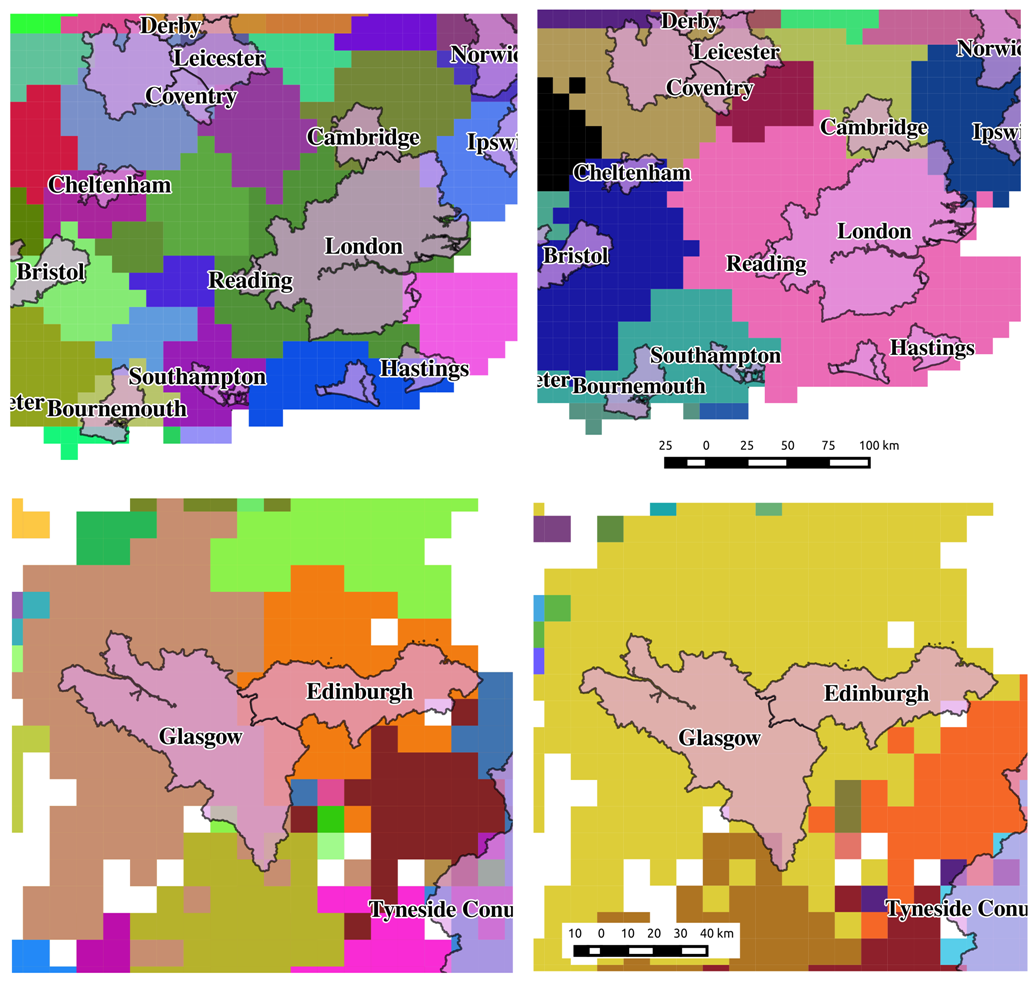
\includegraphics[width=0.7\linewidth]{./figure/PNG/S6_community_london}
\caption{{\bf The natural regions inferred from Twitter user displacements greater than 4 km (left) and 10 km (right) in comparison with major cities in England (upper figures) and Scotland (bottom figures).}  Each color represents a unique community. Including short distance movements has increased the power to differentiate the influence of nearby cities such as Glasgow and Edinburgh (lower left), while restricting the analysis to longer distance movements grouped travelers from the two previous cities into the same community (lower right).}
\label{S6_Fig}
\end{figure}

A more detailed study was conducted over the greater London region revealed by the intra-city spatial interaction patterns.
The space partitions derived from a fine grid of 1km and using all available Twitter user trips without any restriction on the trip’ distances yielded geographic boundaries comparable to some of London boroughs administrative boundaries (Fig.~\ref{S7_Fig}).
However, some areas showed to be more cohesive and displayed more spatial interactions across the administrative boundaries like the area of central London.
Although, the results suggest that the travelers seems to be localized over certain areas of the city for most of their time, and some regions showed long distance interaction patterns.
For example, the separate geographic areas in the south of Hillingdon marking the domain of Heathrow Airport exhibits more connectivity to central London than to the surrounding which is explained by usual flight passengers routes.
The technique also reveals some of the emerging communities around  borders as a result of spatial intermingling of both communities across the borders.
For example, East Barnet and West Enfield seems to have higher interaction that resulted in the emerging cohesive zone between the two boroughs.

\begin{figure}[ht]
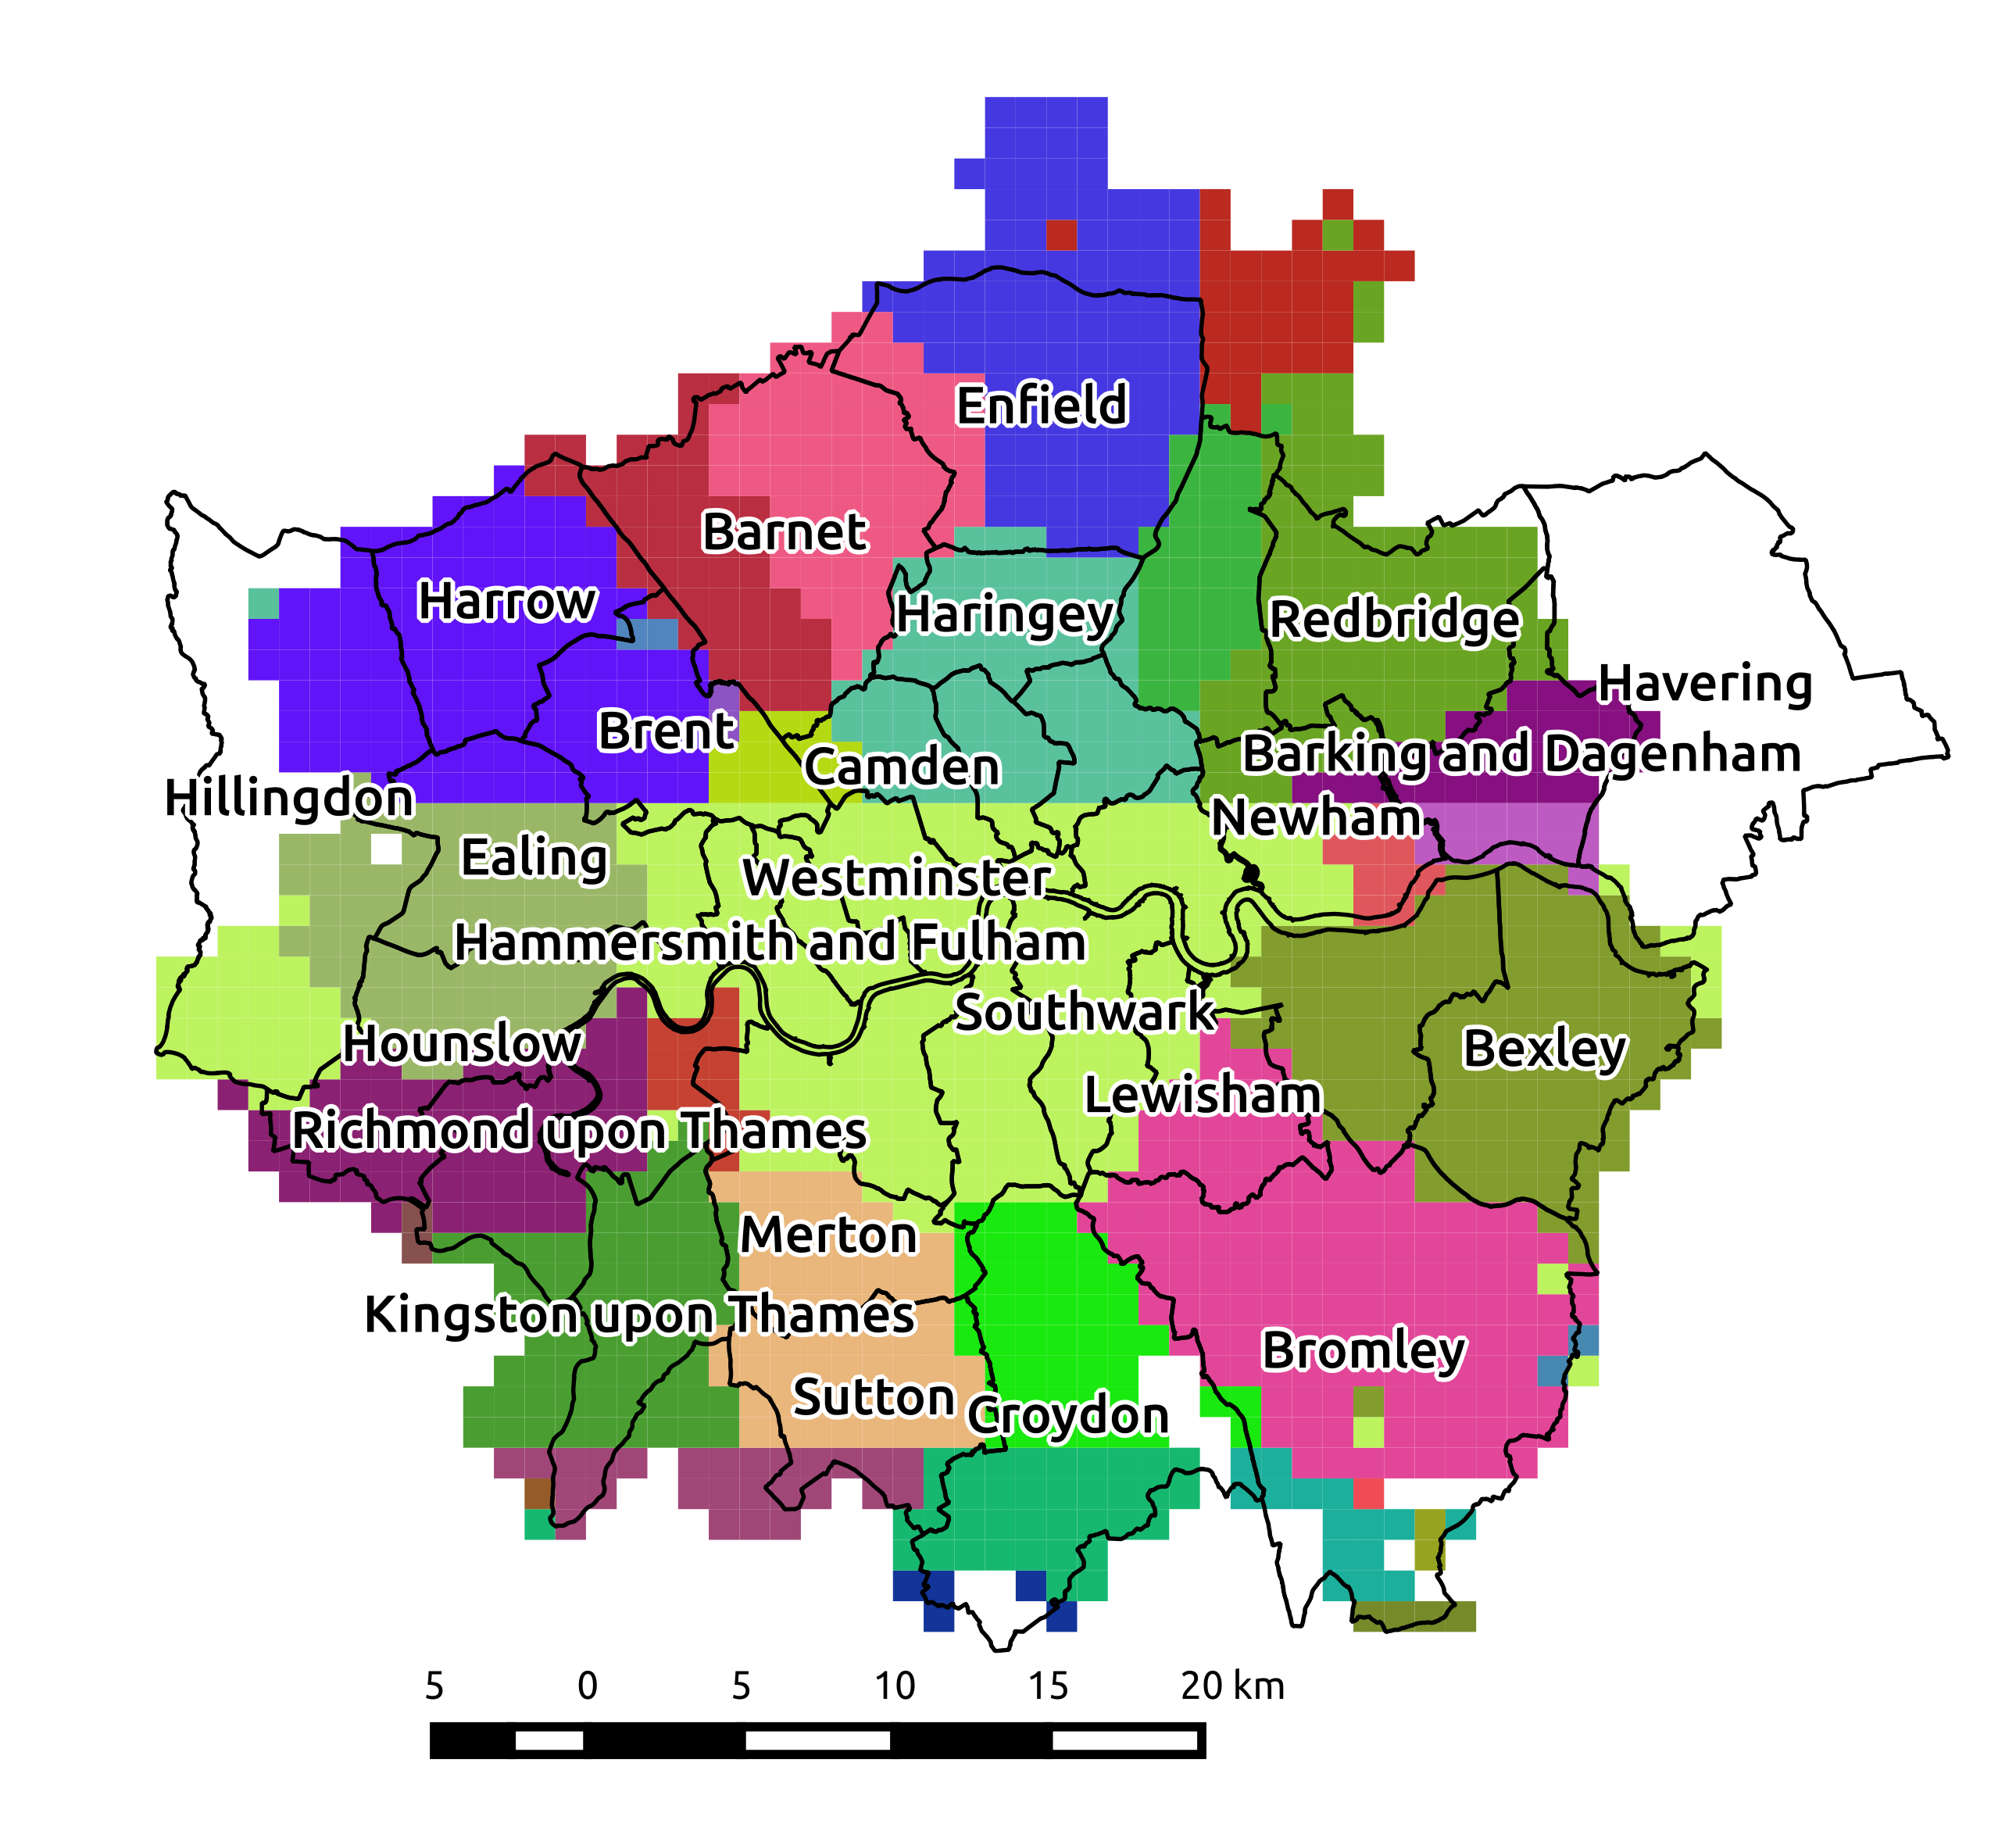
\includegraphics[width=0.8\linewidth]{./figure/PNG/S7_london}
\caption{{\bf Natural boundaries inferred from collective Twitter user displacements in the city of London compared to the boundaries of London boroughs}  A fine fishnet of 1 km cells were used to identify the detailed connectivity patterns based on all the Twitter user displacements in the area.  Each unique color represents a different natural region. Notice that some remote regions like the airport (light green region in south of Hillingdon) share the same class with downtown because it is well connected despite the geographic separation.}
\label{S7_Fig}
\end{figure}


\section*{Conclusion}
In this study,  we delineated the natural urban boundaries in Great Britain from a network of large-scale Twitter user spatial interactions, which are inferred from the collective Twitter user movements extracted from more than 69 million Twitter messages.
In contrast to urban boundaries defined by government agencies with the ``top-down” based approach, we took a ``bottom-up" approach by first imposing a virtual fishnet over the islands of Great Britain, which serves as a proxy to partition the space.
By studying the probability distributions of radius of gyrations of individual Twitters users, we chose 10 km as the cell size, which is the value for quantifying the spatial coverage from majority of Twitter users in Great Britain. 
Twitter user movements were used to establish the connections between the virtual fishnet cells as nodes in a directed weighted network.  
We then applied the map equation algorithm to partition the network,  and associated geographic regions.
The results of strongly connected urban regions in the form of communities in the network space yielded geographically cohesive, non-overlapping urban areas, which provides a clear delineation of the urban boundaries in Great Britain.
By performing statistical analysis of Twitter user mobility patterns in Great Britain, in particular the distribution of collective Twitter user displacements,  we found multi-scale or multi-modal urban movements captured from the Twitter user in Great Britain, which were divided into several distance ranges starting from short intra-city to inter-city movements with clear distinction points.
Identifying the connected regions at each of these distances ranges yielded a hierarchical boundaries of  the urban space in Great Britain.

The power of using Twitter user mobility to delineate natural boundaries is the ability to redraw the city at different mobility ranges inferred objectively from the collective mobility patterns. 
As the urban boundaries are redrawn based on Twitter user movements, which are the physical commuting rather than social ties or phone call initiation, it reflects empirical humans interactions across space.
This study provides a first step in connecting human mobility research with defining natural boundaries, which could assist decision makers regarding resource allocations, political campaigns and urban planning. Finally, as many other mobility datasets, the geo-located twitter data is not able to generalize to the whole population, therefore, the urban regions that do not have any or few Twitter coverage can be missed in the delineation. However, our approach can be still applicable when more detailed mobility data becomes available. 
 
\section*{Acknowledgments}
The authors would like to thank Dr. Kun Zhao and Dr. Raja Jurdak from CSIRO, Australia for their suggestions in generating Figure 1 in this paper. 
The research was supported from National Science Foundation grants No. xx ...

\section*{Author Contribution}
Conceived and designed the experiments: JY AS DY SW. Performed the experiments: JY DY. Analyzed the data: JY AS. Contributed reagents/materials/analysis tools: JY AS DY AS. Wrote the paper: JY AS SW.

\nolinenumbers

\begin{thebibliography}{10}
\bibitem{schliephake}
Schliephake, C., 2014. Urban Ecologies: City Space, Material Agency, and Environmental Politics in Contemporary Culture. Lexington Books.

\bibitem{lynch1960}
Lynch, K., 1960. The image of the city. MIT press.

\bibitem{jiang2015}
Jiang, B., Miao, Y., 2015. The evolution of natural cities from the perspective of location-based social media. The Professional Geographer, 67(2), 295-306.

\bibitem{long2015}
Long, Y., Han, H., Tu, Y., Shu, X., 2015. Evaluating the effectiveness of urban growth boundaries using human mobility and activity records. Cities, 46, 76-84.

\bibitem{liu2015}
Liu, X., Gong, L., Gong, Y., Liu, Y., 2015. Revealing travel patterns and city structure with taxi trip data. J. Transportation Geography, 43, 78–90. doi:10.1016/j.jtrangeo.2015.01.016

\bibitem{lancichinetti2009}
Lancichinetti, A., Fortunato, S., 2009. Community detection algorithms: A comparative analysis. Physical Review E, 80, 056117. doi:10.1103/PhysRevE.80.056117

\bibitem{ratti2010}
Ratti, C., Sobolevsky, S., Calabrese, F., Andris, C., Reades, J., Martino, M., Claxton, R., Strogatz, S.H., 2010. Redrawing the Map of Great Britain from a Network of Human Interactions. PLoS ONE 5, e14248. doi:10.1371/journal.pone.0014248

\bibitem{sobolevsky2013}
Sobolevsky S, Szell M, Campari R, Couronné T, Smoreda Z, Ratti, C., 2013. Delineating Geographical Regions with Networks of Human Interactions in an Extensive Set of Countries. PLoS ONE 8(12): e81707. doi: 10.1371/journal.pone.0081707

\bibitem{kallus2015}
Kallus Z, Barankai N, Szüle J, Vattay G., 2015 Spatial Fingerprints of Community Structure in Human Interaction Network for an Extensive Set of Large-Scale Regions. PLoS ONE 10(5): e0126713. doi: 10.1371/journal.pone.0126713 

\bibitem{hawelka}
Hawelka, B., Sitko, I., Beinat, E., Sobolevsky, S., Kazakopoulos, P., Ratti, C., 2014. Geo-located Twitter as proxy for global mobility patterns. Cartography and Geographic Information Science, 41, 260–271. doi:10.1080/15230406.2014.890072

\bibitem{jurdak2015}
Jurdak, R., Zhao, K., Liu, J., AbouJaoude, M., Cameron, M., Newth, D., 2015. Understanding Human Mobility from Twitter. PLoS ONE 10, e0131469. doi:10.1371/journal.pone.0131469

\bibitem{thiemann}
Thiemann, C., Theis, F., Grady, D., Brune, R., Brockmann, D., 2010. The Structure of Borders in a Small World. PLoS ONE 5, e15422. doi:10.1371/journal.pone.0015422

\bibitem{domenico2015}
De Domenico, M., Lancichinetti, A., Arenas, A., Rosvall, M., 2015. Identifying Modular Flows on Multilayer Networks Reveals Highly Overlapping Organization in Interconnected Systems. Physical Review X, 5. doi:10.1103/PhysRevX.5.011027

\bibitem{fortunato2007}
Fortunato, S., Barthélemy, M., 2007. Resolution limit in community detection. Proceedings of the National Academy of Sciences, 104, 36–41. doi:10.1073/pnas.0605965104

\bibitem{newman2006}
Newman, M.E.J., 2006. Modularity and community structure in networks. Proceedings of the National Academy of Sciences, 103, 8577–82. doi:10.1073/pnas.0601602103

\bibitem{gonzalez2008}
González, M.C., Hidalgo, C.A., Barabási, A.-L., 2008. Understanding individual human mobility patterns. Nature, 453, 779–82. doi:10.1038/nature06958

\bibitem{coscia2011}
Coscia, M., Giannotti, F., Pedreschi, D., 2011. A Classification for Community Discovery Methods in Complex Networks. Statistical Analysis and Data Mining, 4, 512–546. doi:10.1002/sam.10133

\bibitem{rinzivillo2012}
Rinzivillo, S., Mainardi, S., Pezzoni, F., Coscia, M., Pedreschi, D., Giannotti, F., 2012. Discovering the Geographical Borders of Human Mobility. KI - Künstl. Intell. 26, 253–260. doi:10.1007/s13218-012-0181-8

\bibitem{zhong2014}
Zhong, C., Arisona, S.M., Huang, X., Batty, M., Schmitt, G., 2014. Detecting the dynamics of urban structure through spatial network analysis. International Journal of Geographical Information Science, 28, 2178–2199. doi:10.1080/13658816.2014.914521

\bibitem{qian2013}
Qian, W., Stanley, K. G., Osgood, N. D., 2013. The impact of spatial resolution and representation on human mobility predictability. In Web and Wireless Geographical Information Systems,  pp. 25-40, Springer Berlin Heidelberg.

\bibitem{sakaki2010}
Sakaki, T., Okazaki, M., Matsuo, Y., 2010. Earthquake Shakes Twitter Users: Real-time Event Detection by Social Sensors, in: Proceedings of the 19th International Conference on World Wide Web, WWW ’10. ACM, New York, NY, USA, pp. 851–860. doi:10.1145/1772690.1772777

\bibitem{zandbergen2009}
Zandbergen, P.A., 2009. Accuracy of iPhone Locations: A Comparison of Assisted GPS, WiFi and Cellular Positioning. Transactions in GIS, 13, 5–25. doi:10.1111/j.1467-9671.2009.01152.x

\bibitem{liuPopMobility}
Liu, J., Zhao, K., Khan, S., Cameron, M., Jurdak, R., 2014. Multi-scale Population and Mobility Estimation with Geo-tagged Tweets. ArXiv14120327 Phys.

\bibitem{openshaw1984}
Openshaw, S., 1984. The modifiable areal unit problem. Geo Abstracts University of East Anglia.

\bibitem{wong2009}
Wong, D., 2009. The modifiable areal unit problem (MAUP). SAGE Publications: London, UK.

\bibitem{brockmann2006}
Brockmann, D., Hufnagel, L., Geisel, T., 2006. The scaling laws of human travel. Nature 439, 462–5. doi:10.1038/nature04292

\bibitem{song2012}
Song, C., Wang, D., Barabási, A.-L., 2012. Connections between human dynamics and network science. ArXiv Prepr. ArXiv12091411.

\bibitem{guimera2004}
Guimerà, R., Sales-Pardo, M., Amaral, L.A.N., 2004. Modularity from fluctuations in random graphs and complex networks. Physical Review E, 70, 025101. doi:10.1103/PhysRevE.70.025101

\bibitem{good2010}
Good, B.H., de Montjoye, Y.-A., Clauset, A., 2010. Performance of modularity maximization in practical contexts. Physical Review E, 81, 046106. doi:10.1103/PhysRevE.81.046106

\bibitem{rosvall2008}
Rosvall, M., Bergstrom, C.T., 2008. Maps of random walks on complex networks reveal community structure. Proceedings of the National Academy of Sciences, 105, 1118–1123.

\bibitem{rosvall2010}
Rosvall, M., Axelsson, D., Bergstrom, C.T., 2010. The map equation. The European Physical Journal Special Topics, 178, 13–23. doi:10.1140/epjst/e2010-01179-1

\bibitem{clauset2009}
Clauset, A., Shalizi, C., Newman, M., 2009. Power-Law Distributions in Empirical Data. Society for Industrial and Applied Mathematics Review. 51, 661–703. doi:10.1137/070710111


\bibitem{rhee2011}
Rhee, I., Shin, M., Hong, S., Lee, K., Kim, S. J., and Chong, S., 2011. On the levy-walk nature of human mobility. IEEE/ACM transactions on networking (TON), 19(3), 630-643.

\bibitem{reynolds2012}
Reynolds, A., 2012. Truncated levy walks are expected beyond the scale of data collection when correlated random walks embody observed movement patterns. Journal of The Royal Society Interface, 9(68), 528-534.

\bibitem{zhao2015}
Zhao, K., Musolesi, M., Hui, P., Rao, W., and Tarkoma, S., 2015. Explaining the power-law distribution of human mobility through transportation modality decomposition. Scientific reports, 5.

\bibitem{simini2012}
Simini, F., González, M. C., Maritan, A., Barabási, A. L., 2012. A universal model for mobility and migration patterns. Nature, 484(7392), 96-100.

%\bibitem{blondel2008}
%Blondel, V.D., Guillaume, J., Lambiotte, R., Lefebvre, E., 2008. Fast unfolding of community hierarchies in large networks. Networks 1–6.
%

\end{thebibliography}
\end{document}

